% Created 2021-01-24 Sun 22:50
% Intended LaTeX compiler: pdflatex
\documentclass[11pt]{article}
\usepackage[utf8]{inputenc}
\usepackage[T1]{fontenc}
\usepackage{graphicx}
\usepackage{grffile}
\usepackage{longtable}
\usepackage{wrapfig}
\usepackage{rotating}
\usepackage[normalem]{ulem}
\usepackage{amsmath}
\usepackage{textcomp}
\usepackage{amssymb}
\usepackage{capt-of}
\usepackage{hyperref}
\usepackage{minted}
\hypersetup{colorlinks=true, linkcolor=black, filecolor=red, urlcolor=blue}
\usepackage[turkish]{babel}
\author{Eren Hatırnaz}
\date{8 Eylül 2019}
\title{Yazılım Gündemi - 8\\\medskip
\large 2-8 Eylül 2019}
\hypersetup{
 pdfauthor={Eren Hatırnaz},
 pdftitle={Yazılım Gündemi - 8},
 pdfkeywords={},
 pdfsubject={},
 pdfcreator={Emacs 27.1 (Org mode 9.3)},
 pdflang={Turkish}}
\begin{document}

\maketitle
\tableofcontents \clearpage\shorthandoff{=}

\begin{center}
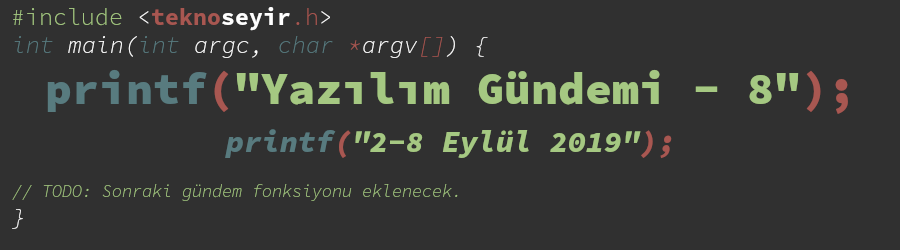
\includegraphics[width=.9\linewidth]{gorseller/yazilim-gundemi-banner.png}
\end{center}

\begin{center}
\href{../07/yazilim-gundemi-07.pdf}{< Önceki Gündem} | \textbf{2-8 Eylül 2019} | \href{../09/yazilim-gundemi-09.pdf}{Sonraki Gündem >}

\href{https://teknoseyir.com/blog/yazilim-gundemi-8-2-8-eylul-2019}{TeknoSeyir'de Oku}
\end{center}

\section{IEEE Spectrum, \href{https://spectrum.ieee.org/computing/software/the-top-programming-languages-2019}{popüler ilk 10 programlama dili listesi}ni yayınlandı}
\label{sec:org7a0d9b7}
Amerika'da yer alan Institute of Electrical and Electronics Engineers
(Elektrik ve Elektronik Mühendisleri Enstitüsü) tarafından her yıl yayınlanan
"en popüler 10 programlama dili" listesinin 2019 sürümü bu hafta yayınlandı.
Liste sıralaması bu şekilde:

\begin{center}
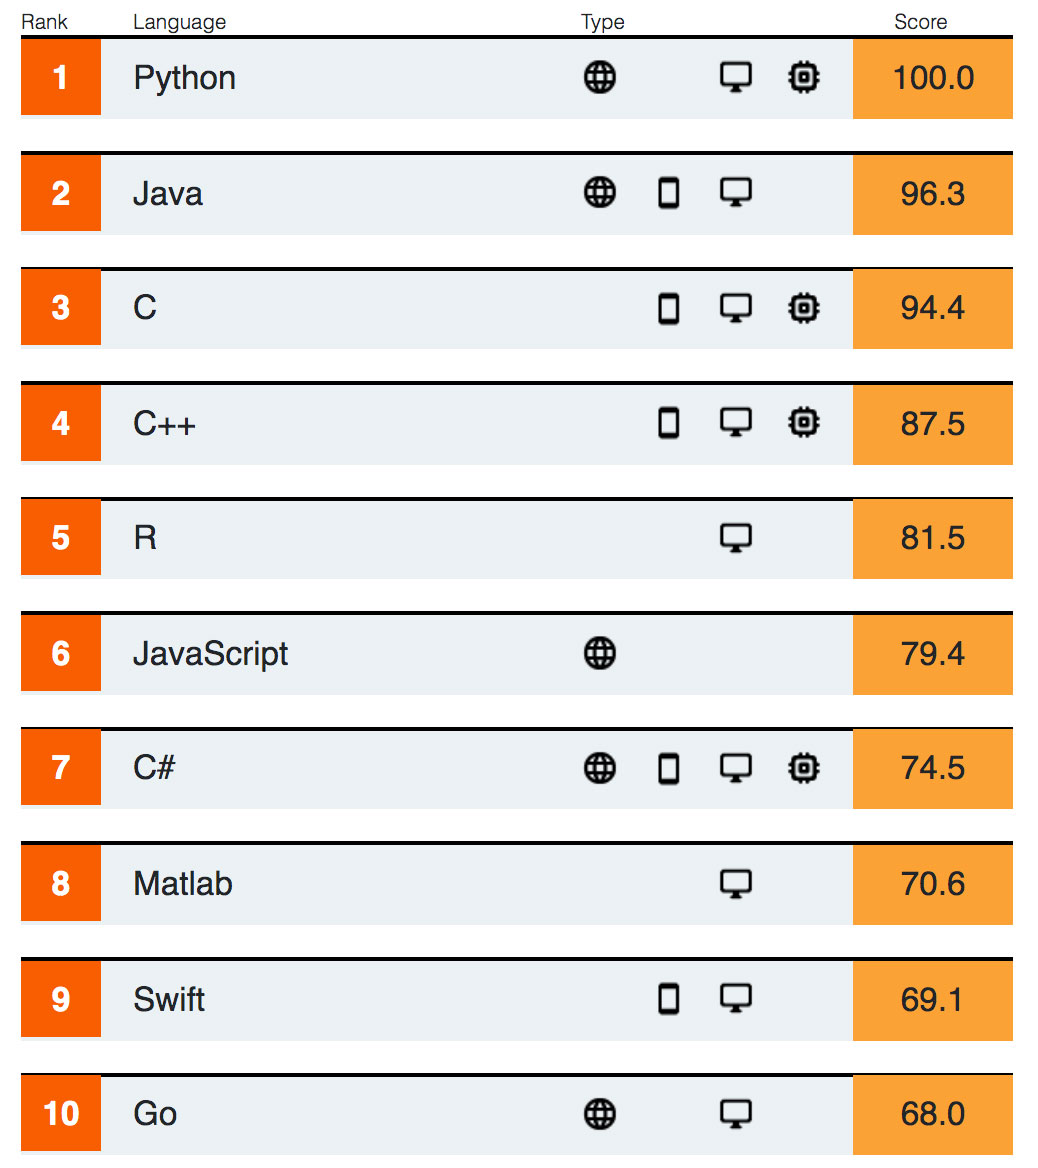
\includegraphics[height=6cm]{gorseller/populer-10-programlama-dili.png}
\end{center}

Listenin filtrelenebilir hali ve devamı için \href{https://spectrum.ieee.org/static/interactive-the-top-programming-languages-2019}{bu sayfaya} göz atabilirsiniz.
\section{COBOL programlama dili \href{https://www.zdnet.com/article/cobol-turns-60-why-it-will-outlive-us-all/}{60 yaşında}}
\label{sec:org1555711}
İlk olarak 1959 duyurulan COBOL programlama dili bu hafta itibariyle 60.yaşını
doldurdu. Ben dahil yazıyı okuyan herkesten daha büyük olduğu için hakkında pek
bilgiye sahip değilim fakat konu başlığına eklediğim bağlantıdaki habere göre
basit söz dizimi (syntax) sayesinde diğer programlama dillerinden öne
çıkabilmiş. Haberde benim ilginçime giden programlama dilinin yaratıcılarının
destek ve potansiyel müşteri bulabilmeleri için 41 bilgisayar üreticisi ile
Pentagon'da \href{https://ieeexplore.ieee.org/document/4640600?reload=true}{Committee of the Conference on Data Systems Languages (CODASYL)}
isimli konferansta toplantı yapması ve programlama dilinin isminin de orada
konulması. Yoksa COBOL bir Pentagon projesi mi?! :) Neyse şaka bir yana,
programlama tarihiyle ilgili arkadaşların konu başlığındaki yazıyı okumalarını
tavsiye ederim. İleri bir okuma için de, COBOL'un 60 yaşına gelebilmesini
sağlayan 6 neden başlıklı \href{https://www.eweek.com/development/six-reasons-cobol-has-survived-to-age-60}{şu yazı} okunabilir.
\section{Laravel \href{https://laravel-news.com/laravel-6}{6 sürümü yayınlandı}}
\label{sec:orgee54dbe}
Popüler PHP web framework sistemi olan Laravel, 6 numaralı LTS (Long-Term
Support - Uzun dönemli destek) sürümünü bu hafta içerisinde duyurdu. Ayrıca bir
önceki LTS sürümü olan 5.5 sürümünün de 30 Ağustos 2019 itibariyle hata çözme
güncellemesini almayacağını fakat güvenlik güncelleştirmeleri almaya 30 Ağustos
2020'ye kadar devam edeceği bilgisi de duyuru yazısında yer aldı. Laravel 6 ile
gelen bazı özellikler ise şu şekilde:

\begin{itemize}
\item Yetkilendirme cevapları geliştirilmiş: Önceden son kullanıcıya özel hata
mesajları göstermek zormuş fakat bu sürümde \texttt{Gate::inspect} fonksiyonu
eklenerek bu çözülmüş. Örnek kullanım için konu başlığındaki bağlantıya
tıklayabilirsiniz.
\item Laravel 5.x numaralı sürümlerle birlikte gelen UI özellikleri artık
\href{https://github.com/laravel/ui}{laravel/ui} isimli ayrı bir proje haline geldi. Kullanmak için özel olarak
eklemeniz gerekiyor.
\item \href{https://laravel-news.com/job-middleware-is-coming-to-laravel-6}{Job Middleware}
\item \href{https://laravel.com/docs/6.0/collections\#lazy-collections}{Lazy Collections}
\end{itemize}

Diğer değişiklikler ve yenilikler için konu başlığına eklediğim bağlantıya
tıklayabilir ya da bu bağlantıları inceleyebilirsiniz:
\begin{itemize}
\item \href{https://laravel.com/docs/6.0/releases}{Laravel 6 Sürüm Notları}
\item \href{https://laravel.com/docs/6.0/upgrade}{Laravel 6 Yükseltme Rehberi}
\item \href{https://laravel-news.com/laravel-6}{Laravel 6 Katkı Sağlama Rehberi}
\end{itemize}
\section{Mikrokontrolcüler için Qt kütüphanesi webineri düzenlendi}
\label{sec:orgbfe3b99}
\href{../06/yazilim-gundemi-06.pdf}{Yazılım Gündemi - 6} yazısında haberini yaptığım kütüphanenin bu hafta
içerisinde webineri (sanal seminer) düzenlendi ve bazı detaylara yer verildi.
Webinere kayıt olup izlemek istemiştim fakat kurumsal bir e-posta adresi ve
şirket ismi gerekiyordu. Şu an bir şirkette çalışmadığım için kayıt olamadım
fakat \href{https://teknoseyir.com/u/cemkoc}{Cem Koç} arkadaşımız kayıt olmuş ve şu şekilde bazı notlar almış:

\begin{itemize}
\item Cortex-m için rtems üzerine Qt Lite kullanılıyor.
\item Cortex-a için Linux tabanı sistemler üzerine inşaa edilecek. Ama burada Qt
Lite yerine Qt kullanılıyor.
\item Qt for MCUs sadece ticari lisanslanacak. Açık kaynak versiyonu yok. Üzdü
açıkçası.
\item Webinar'da bir uygulama derlendi. Çok basitçe yaptılar gerçekten.
Uygulamayı masaüstü programı olarak test edip direkt binary oluşturacak
gibi sadece hedefi değiştirerek derlenebiliyor. Klasik Qt.
\end{itemize}

Yine \href{https://teknoseyir.com/u/cemkoc}{Cem Koç} hocanın Webiner'den aldığı bazı ekran görüntüleri:

\begin{center}
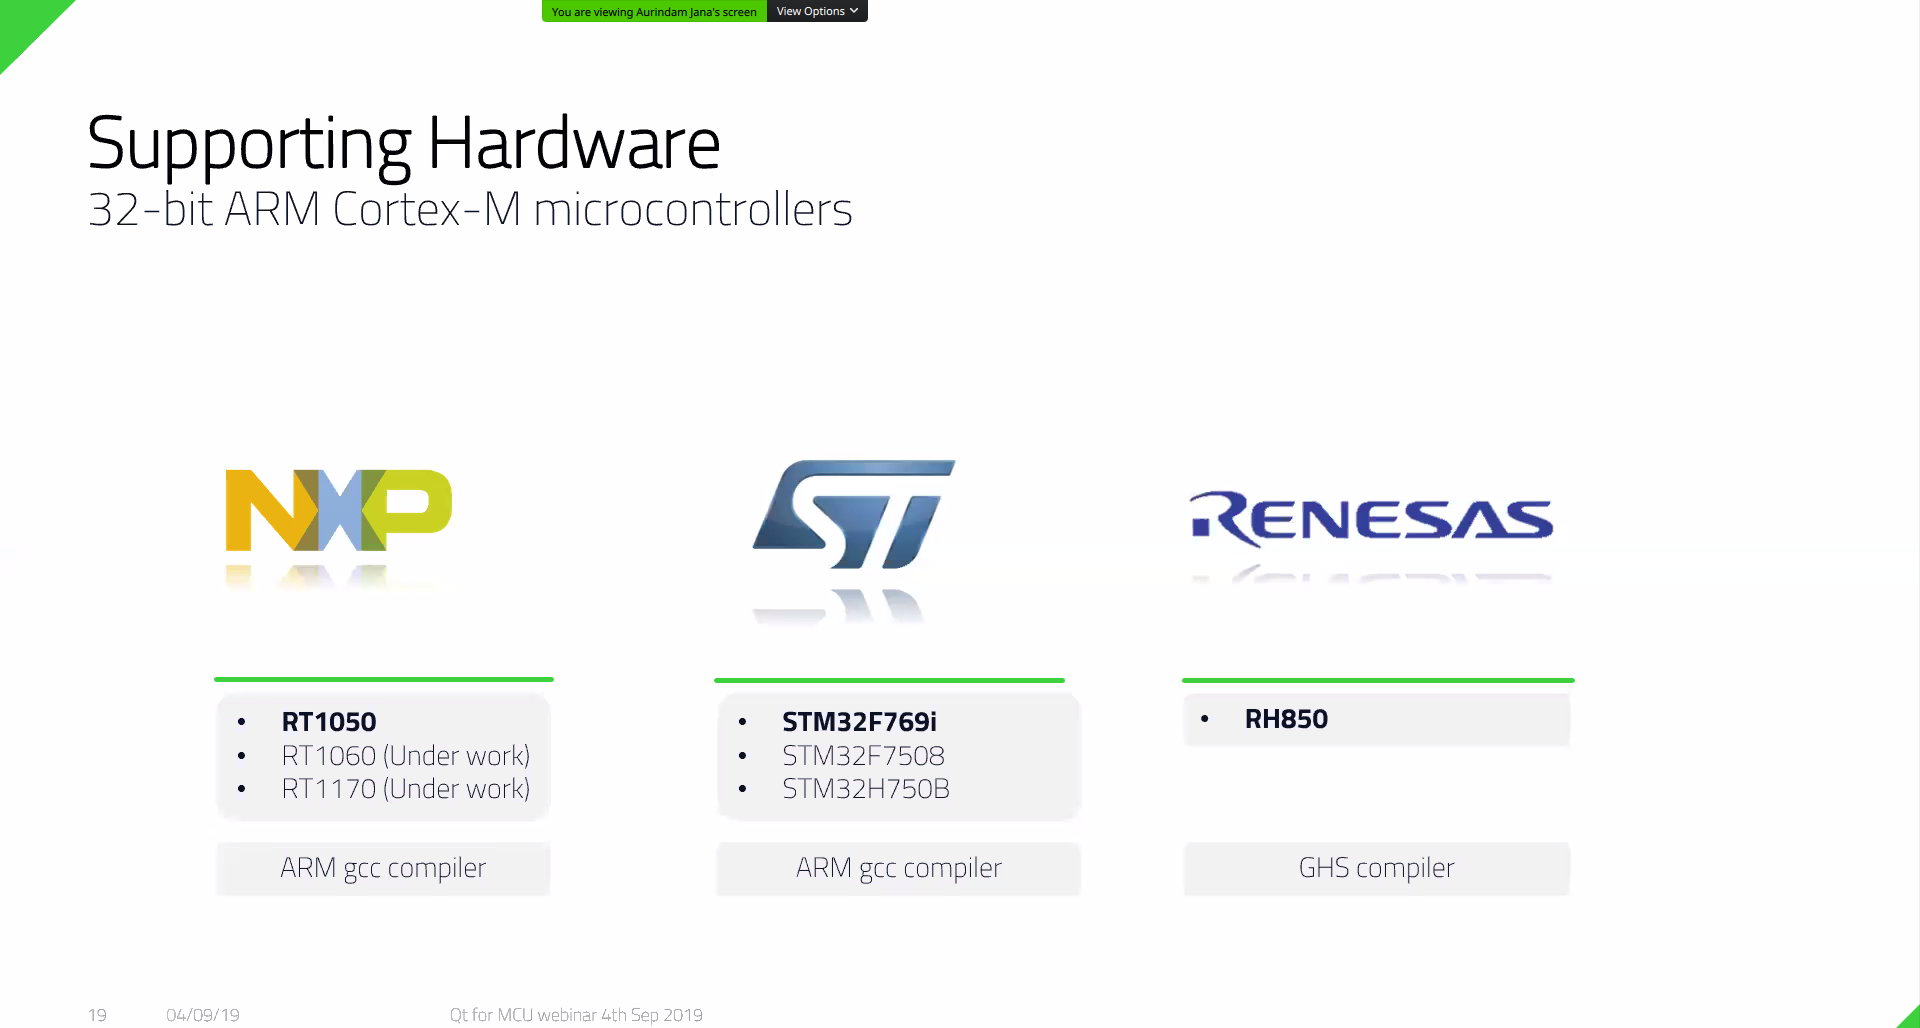
\includegraphics[width=.9\linewidth]{gorseller/qt1.png}
\end{center}
\begin{center}
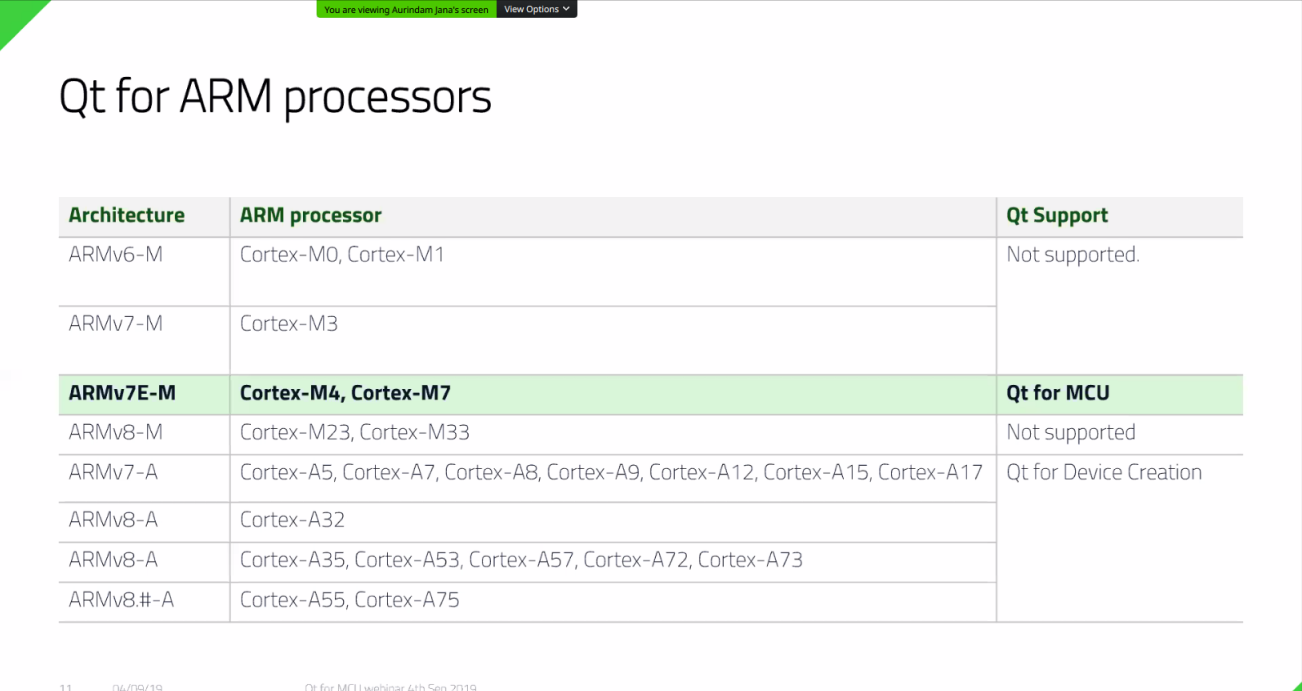
\includegraphics[width=.9\linewidth]{gorseller/qt2.png}
\end{center}
\begin{center}
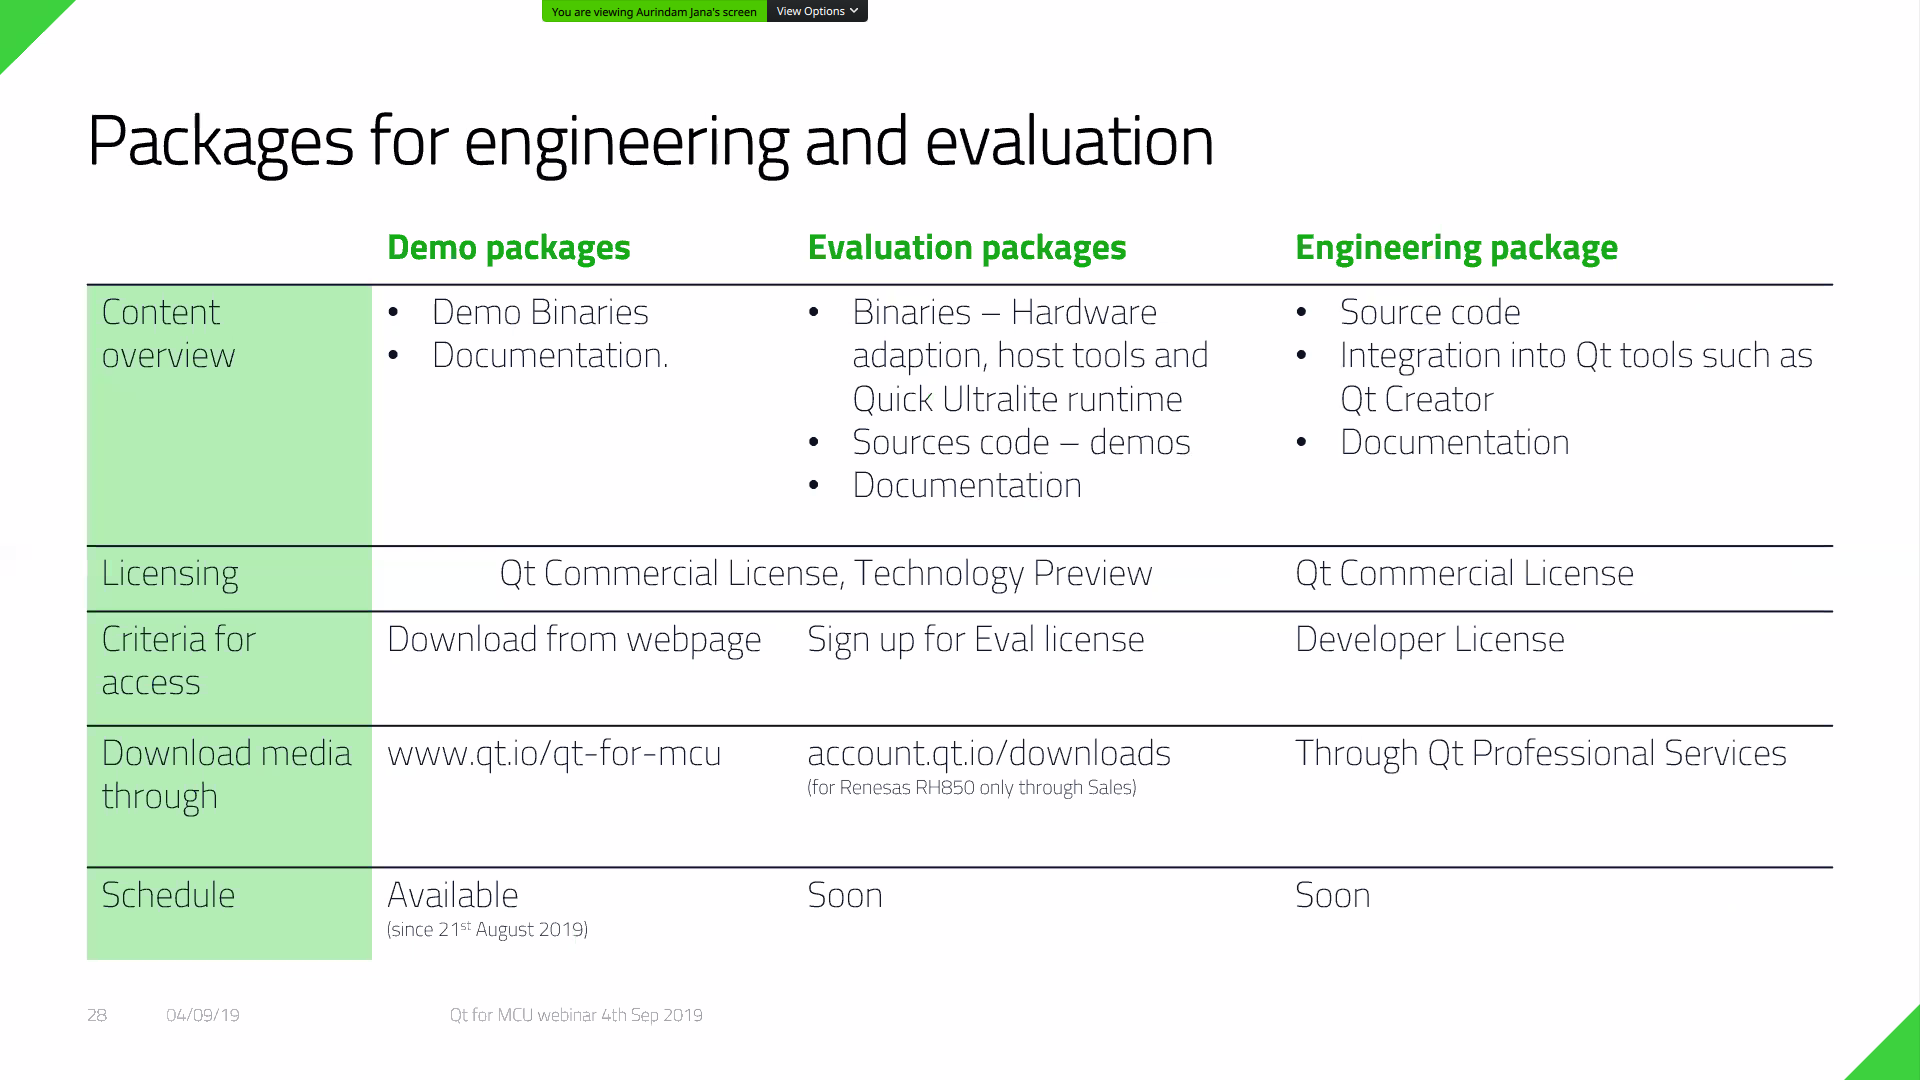
\includegraphics[width=.9\linewidth]{gorseller/qt3.png}
\end{center}
\begin{center}
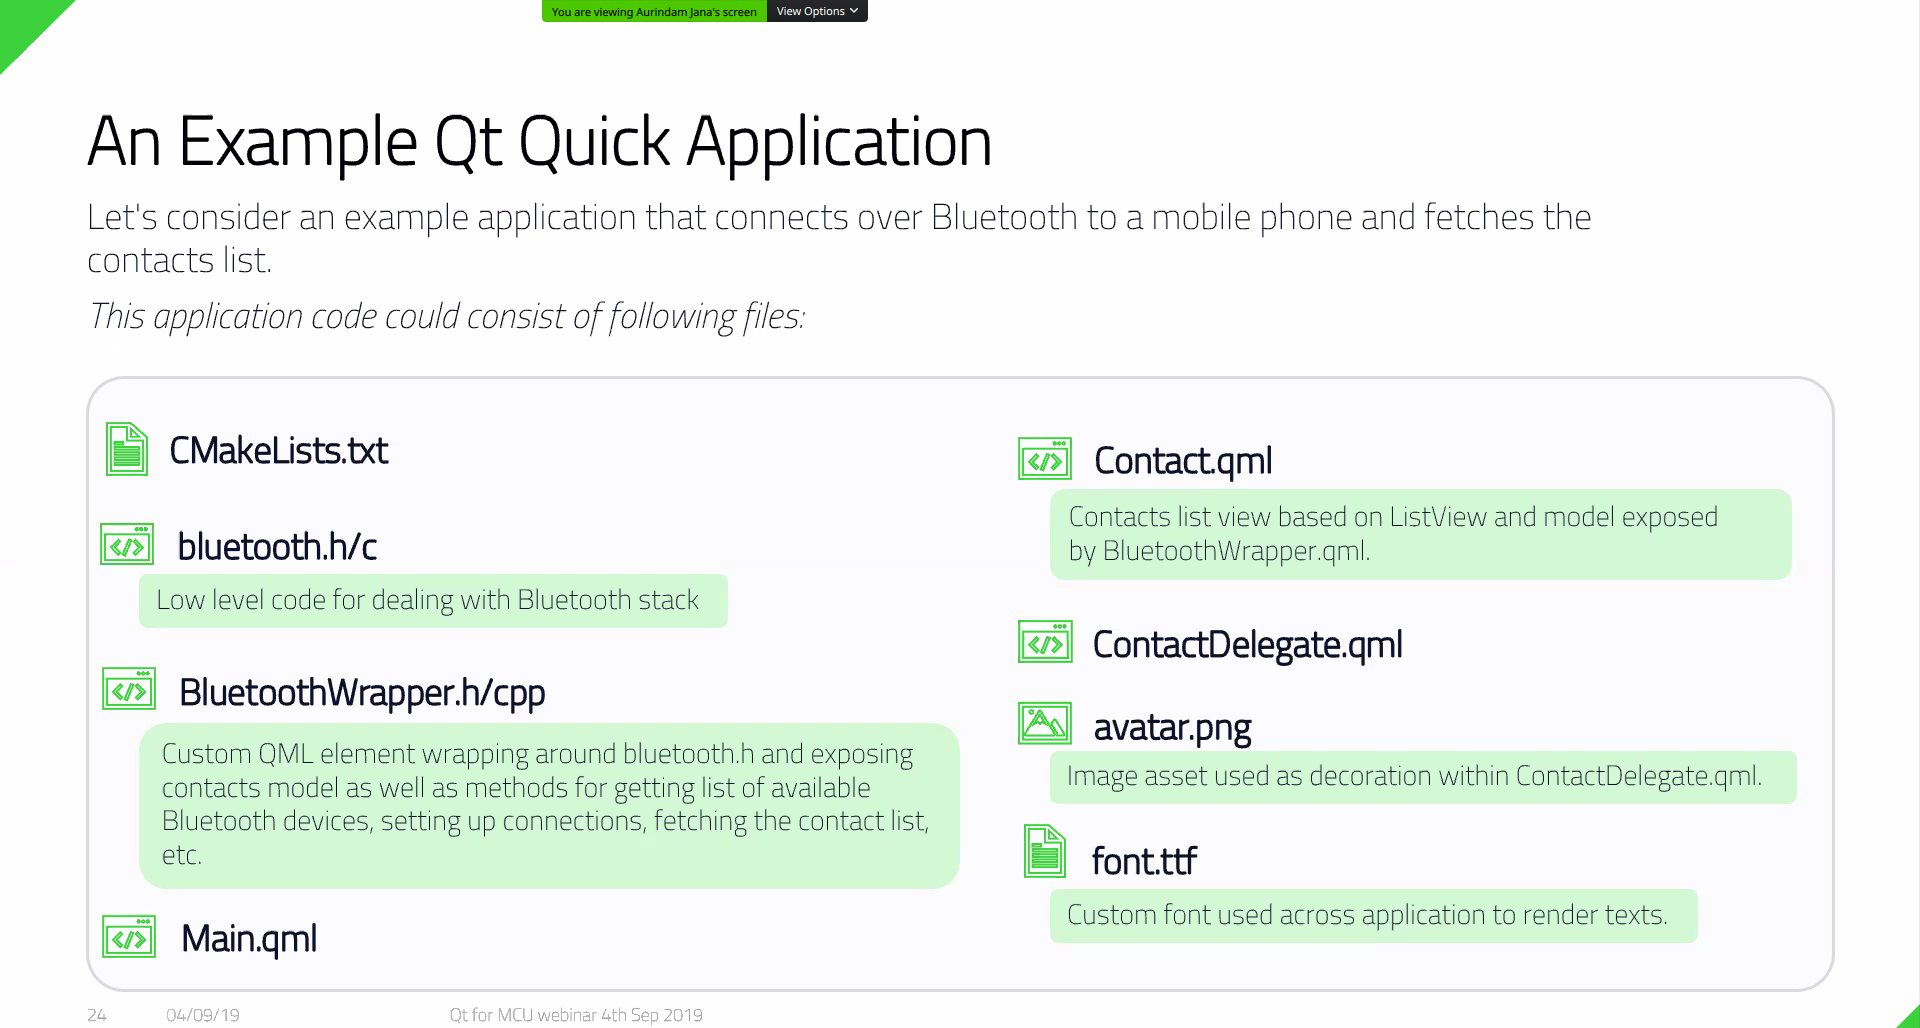
\includegraphics[width=.9\linewidth]{gorseller/qt4.png}
\end{center}
\begin{center}
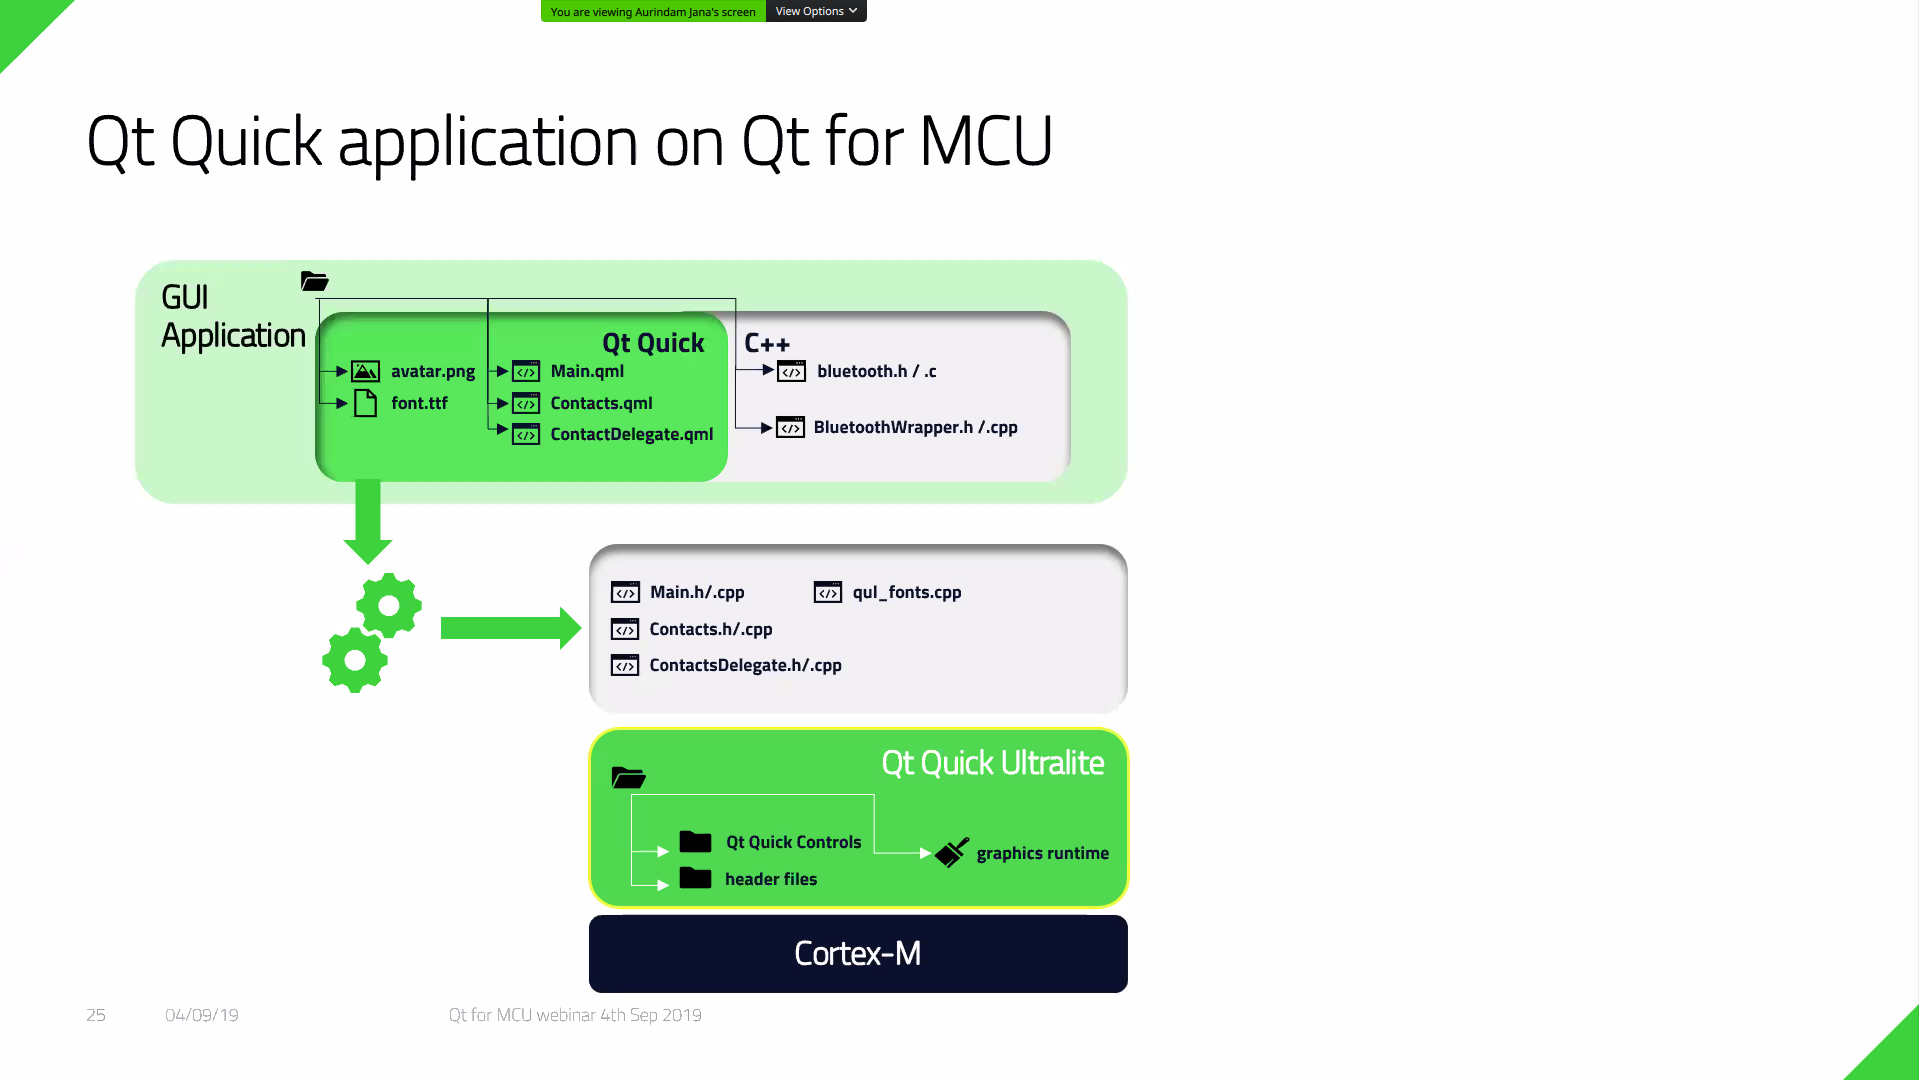
\includegraphics[width=.9\linewidth]{gorseller/qt5.png}
\end{center}
\begin{center}
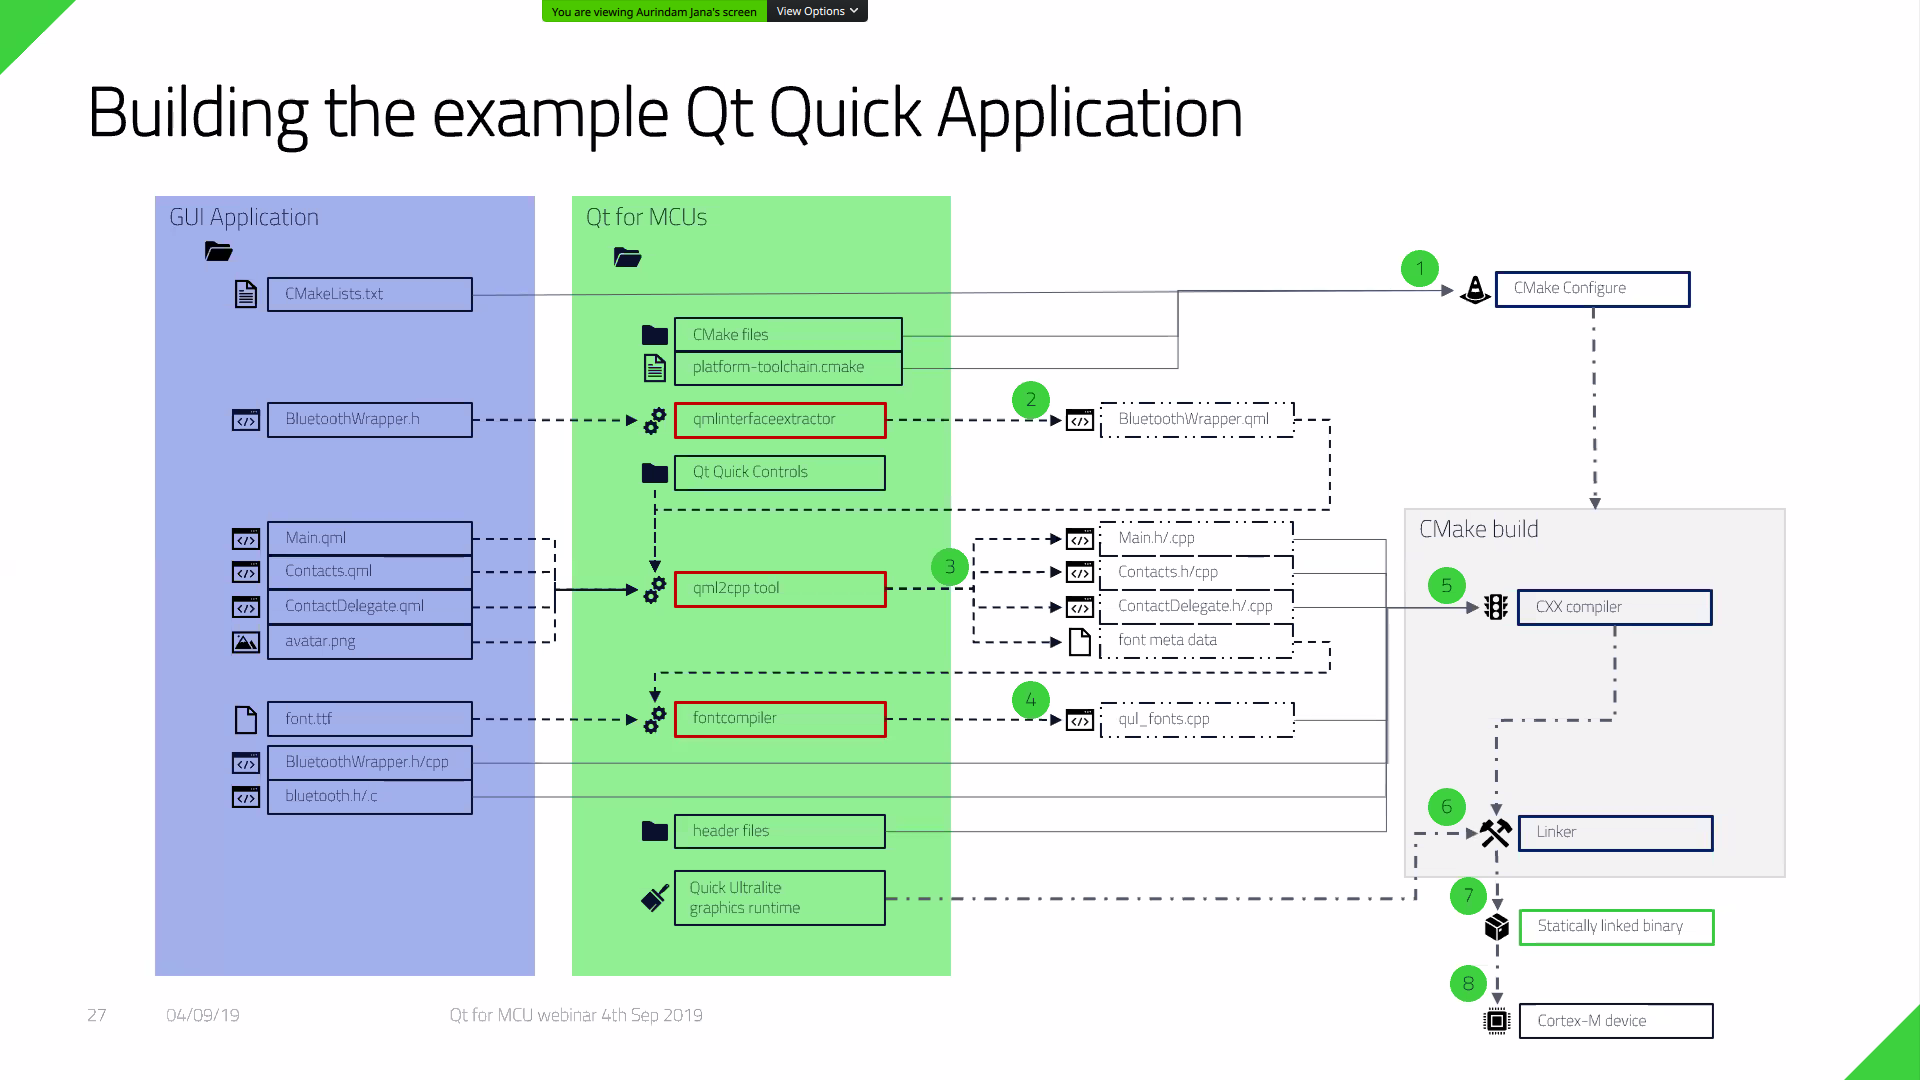
\includegraphics[width=.9\linewidth]{gorseller/qt6.png}
\end{center}
\begin{center}
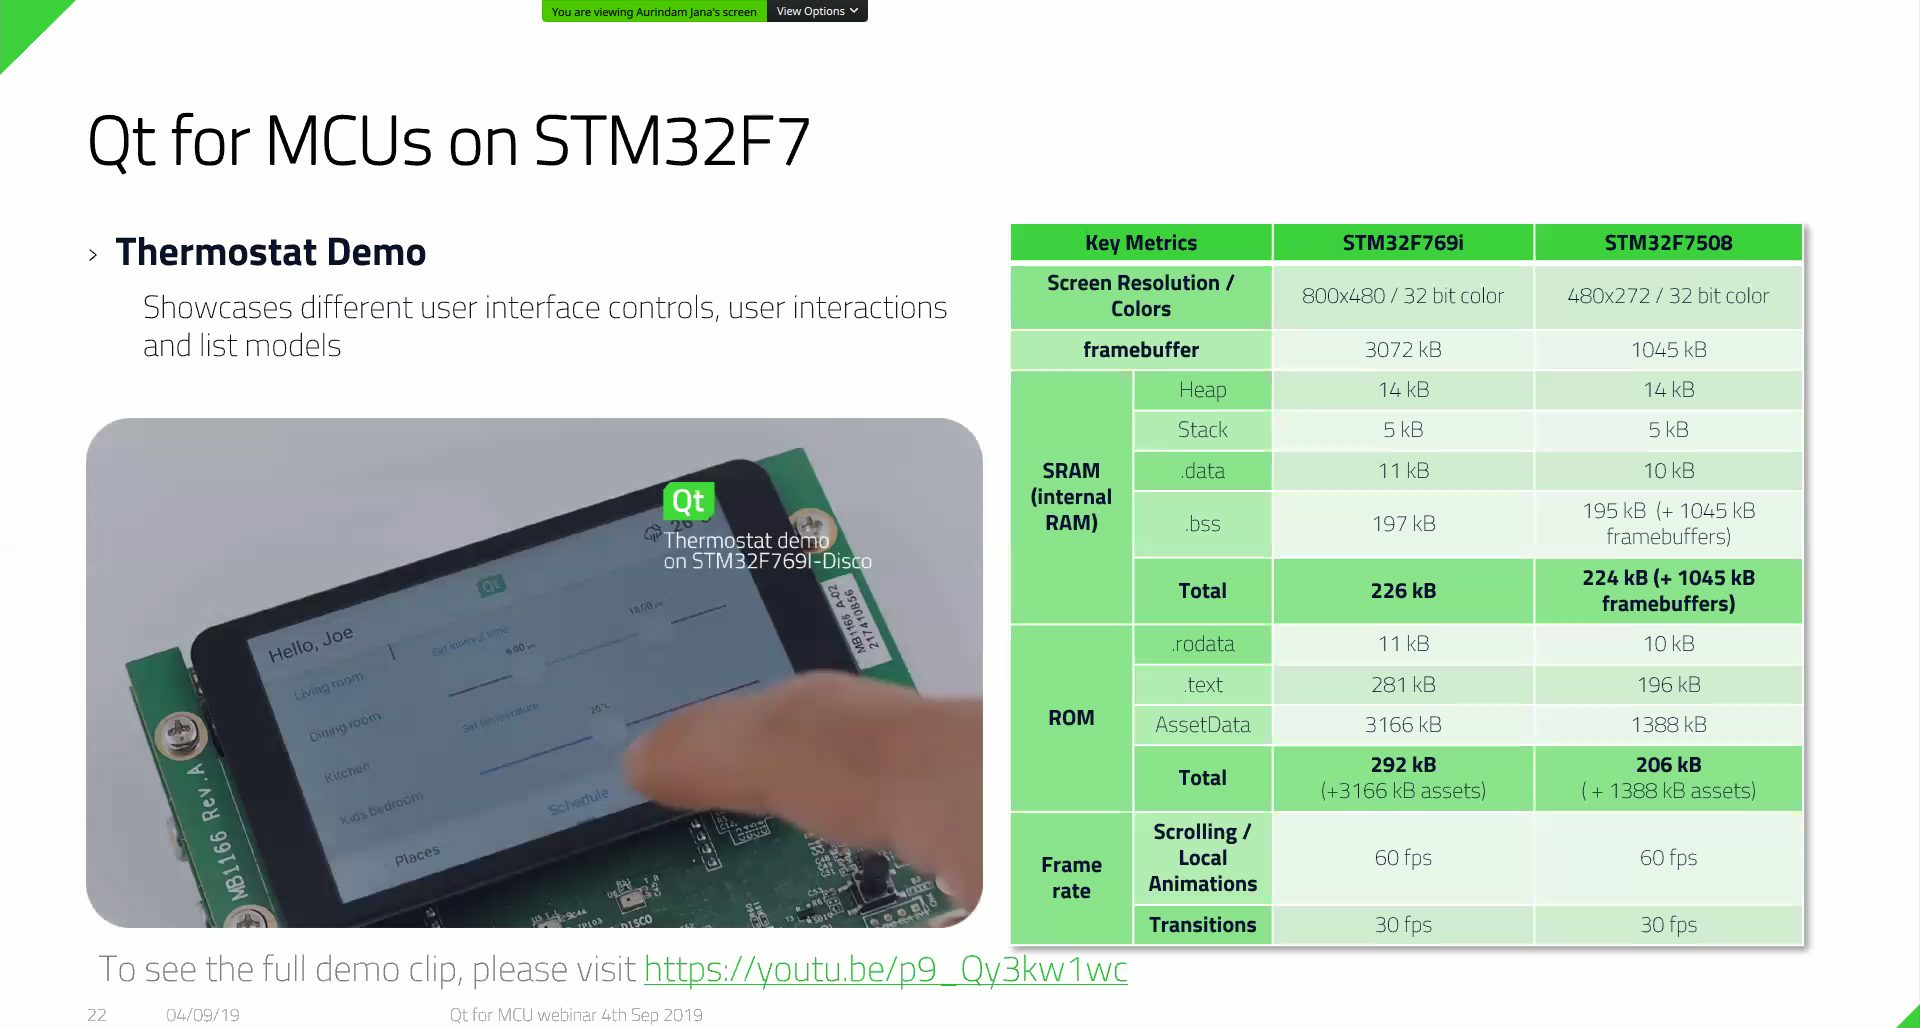
\includegraphics[width=.9\linewidth]{gorseller/qt7.png}
\end{center}
\begin{center}
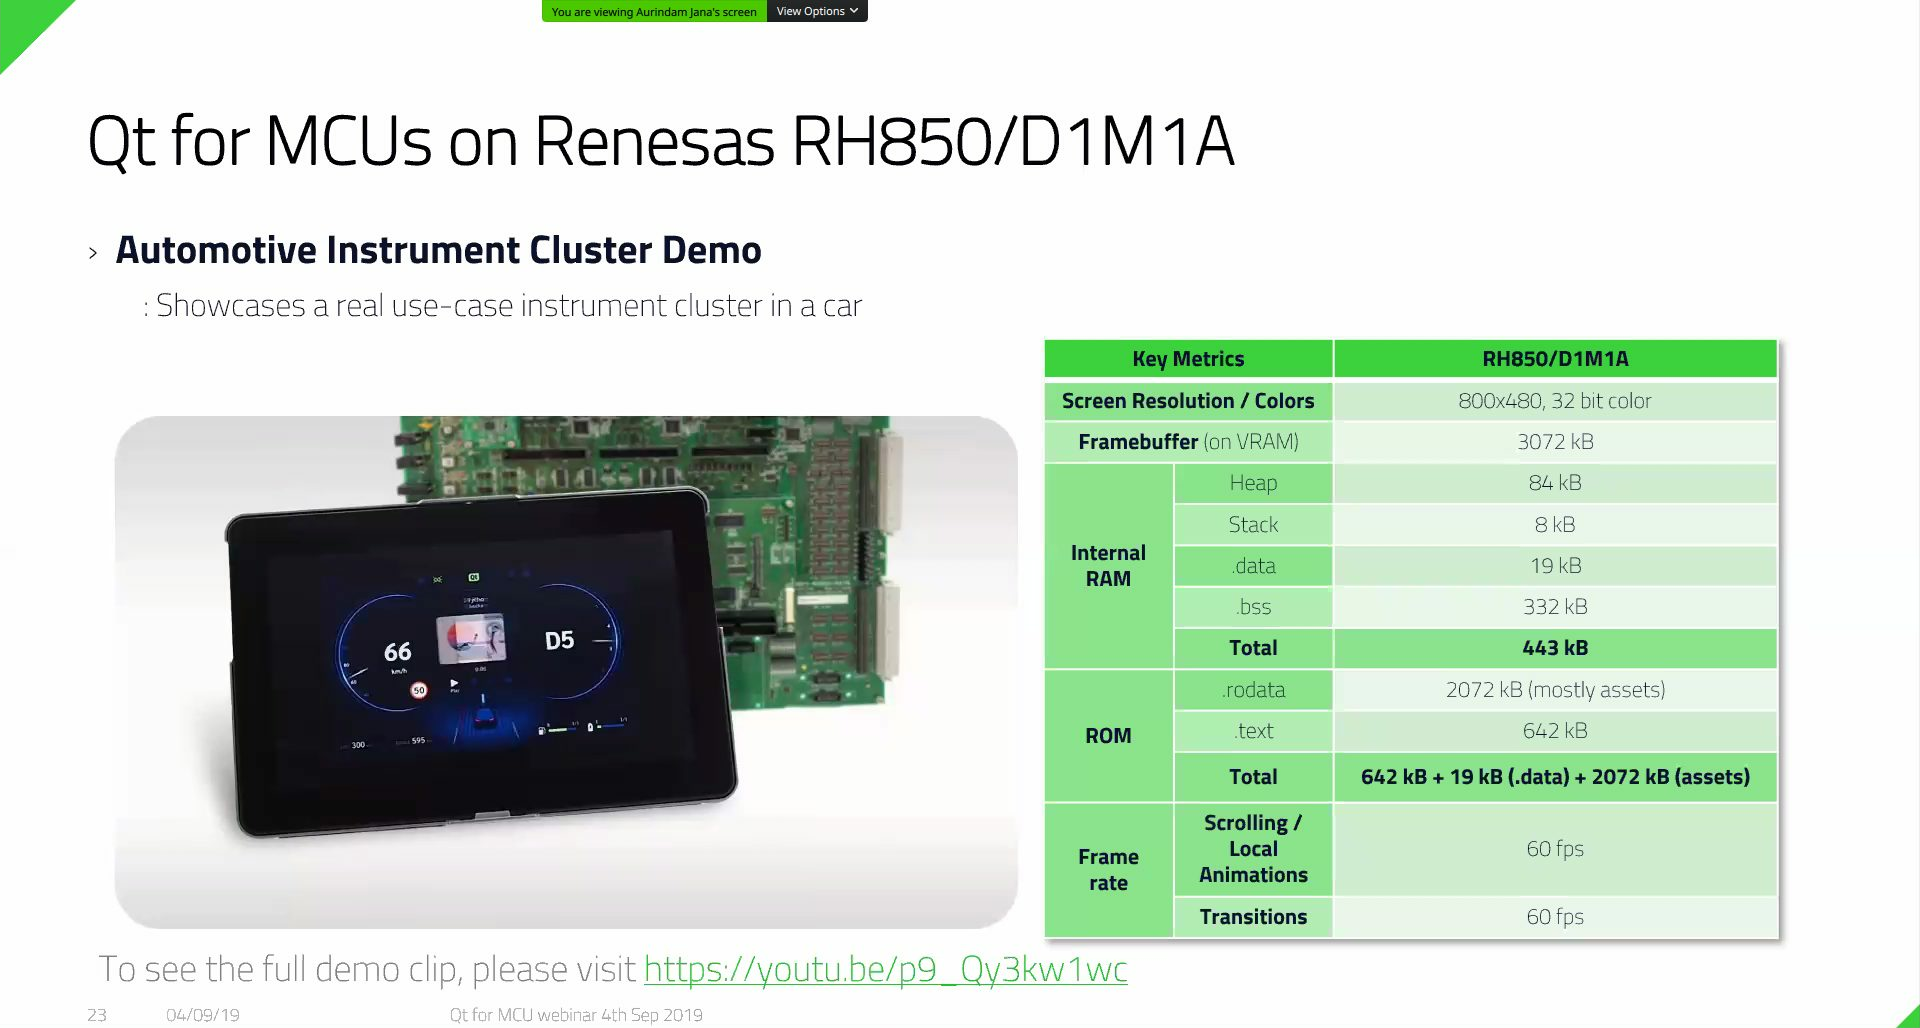
\includegraphics[width=.9\linewidth]{gorseller/qt8.png}
\end{center}

Webiner kaydı daha sonra \href{https://www.youtube.com/watch?v=60cAwGQ\_E7o}{bu adreste} yayınlanmış. Benim izleyecek vaktim olmadı
fakat ilgili arkadaşları mutlaka bakmalarını tavsiye ederim.
\section{Visual Studio Code \href{https://code.visualstudio.com/updates/v1\_38}{1.38 (Ağustos 2019) sürümü yayınlandı}}
\label{sec:org98c2d7c}
\begin{center}
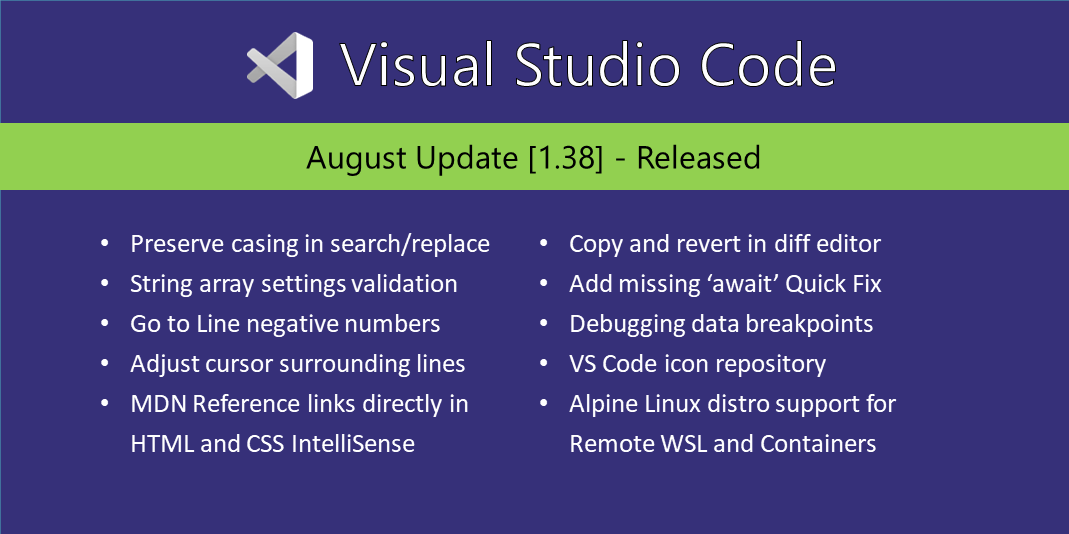
\includegraphics[width=.9\linewidth]{gorseller/vscode1-38.png}
\end{center}
\section{Diğer Haberler}
\label{sec:org6174593}
\begin{itemize}
\item Apple'ın AppStore'daki bazı uygulamaların \href{https://www.washingtonpost.com/technology/2019/09/05/how-apple-uses-its-app-store-copy-best-ideas/?noredirect=on}{fikirlerini kopyaladığı dair
iddialar var}.
\item Google, \href{https://google.github.io/eng-practices/review/}{kod review süreçleriyle ilgili} rehber hazırladı.
\item Google, akademik araştırmalar için yeni bir veri gizliliği teknolojisi
duyurdu: \href{https://developers.googleblog.com/2019/09/enabling-developers-and-organizations.html}{Differential Privacy}. \href{https://developers.googleblog.com/2019/09/enabling-developers-and-organizations.html}{GitHub Deposu}
\item WinUI \href{https://twitter.com/dotMorten/status/1168218666619375616}{API sisteminde değişiklikler} var.
\item Securitum takımı, yeni HTML elementi \href{https://web.dev/hands-on-portals}{portal} hakkında \href{https://research.securitum.com/security-analysis-of-portal-element/}{güvenlik analizi yazısı
yayınlandı}.
\item PHP topluluğu, \texttt{Union Types} özelliğini \href{https://github.com/php/php-rfcs/pull/1}{tartışıyor}.
\item PHP programlama dilinin \href{https://www.php.net/archive/2019.php\#2019-09-05-1}{7.4.0 RC1 sürümü yayınlandı}.
\item Go programlama dilinin \href{https://golang.org/doc/go1.13}{1.13 sürümü duyuruldu}.
\item D programlama dilinin \href{https://dlang.org/blog/2019/09/06/dmd-2-088-0-released/}{2.088.0 sürümü yayınlandı}.
\item Mozilla, Manifest V3 hakkında \href{https://blog.mozilla.org/addons/2019/09/03/mozillas-manifest-v3-faq/}{sıkça sorulan sorular yazısı} yayınlandı.
\item Frontend geliştiriciler için açık kaynak backend sunucusu aracı \href{https://medium.com/eldadfux/introducing-appwrite-an-open-source-backend-server-for-mobile-web-developers-4be70731575d}{açık kaynak
olarak yayınlandı}: \href{https://appwrite.io/}{AppWrite}, \href{https://github.com/appwrite/appwrite}{GitHub Deposu}.
\item AITO firması, yapay zeka destekli yeni bir veritabanı türü tanıttı:
\href{https://aito.ai/blog/introducing-a-new-database-category-the-predictive-database/}{Predictive Database}.
\item Python ile terminal bazlı kullanıcı arayüzleri geliştirmeye yarayan toot
kütüphanesi \href{https://github.com/ihabunek/toot/releases/tag/0.23.0}{0.23.0 sürümünü duyurdu}. \href{https://github.com/ihabunek/toot/blob/master/CHANGELOG.md}{Değişiklik Notları}, \href{https://asciinema.org/a/fTq6pzFOIrPzaIt1ralRM86wE}{Demo}.
\item YugaByte DB \href{https://jepsen.io/analyses/yugabyte-db-1.3.1}{1.3.1 sürümü duyuruldu}.
\item Quasar Framework \href{https://forum.quasar-framework.org/topic/4234/quasar-1-1-0-released-new-component-qvirtualscroll-many-other-new-things-a-lot-of-improvements-and-fixes/2}{1.1.0 sürümü yayınlandı}, \href{https://github.com/quasarframework/quasar}{GitHub Deposu}.
\end{itemize}
\section{Lisans}
\label{sec:orgf2414b1}
\begin{center}
\begin{center}

\includegraphics[height=1.5cm]{../../../img/CC_BY-NC-SA_4.0.png}
\end{center}

\href{yazilim-gundemi-08.pdf}{Yazılım Gündemi - 8} yazısı \href{https://erenhatirnaz.github.io}{Eren Hatırnaz} tarafından \href{http://creativecommons.org/licenses/by-nc-sa/4.0/}{Creative Commons
Atıf-GayriTicari-AynıLisanslaPaylaş 4.0 Uluslararası Lisansı} (CC BY-NC-SA 4.0)
ile lisanslanmıştır.
\end{center}
\end{document}
